\documentclass{standalone}
\usepackage{tikz}

\begin{document}

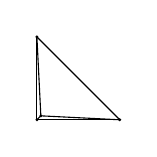
\begin{tikzpicture}[scale=2]
  \node (v0) at (-0.263158, -0.263158) {};
  \fill (v0) circle(0.01);
  \node (v1) at (0.263158, -0.263158) {};
  \fill (v1) circle(0.01);
  \node (v2) at (-0.263158, 0.263158) {};
  \fill (v2) circle(0.01);
  \node (v3) at (-0.238095, -0.238095) {};
  \fill (v3) circle(0.01);
  \draw (v0.center) -- (v1.center);
  \draw (v0.center) -- (v2.center);
  \draw (v0.center) -- (v3.center);
  \draw (v1.center) -- (v2.center);
  \draw (v1.center) -- (v3.center);
  \draw (v2.center) -- (v3.center);
\end{tikzpicture}

\end{document}
